\documentclass[../main.tex]{subfiles}

\subsection{Esettáblázat}
\begin{center}
    \begin{longtable}{| m{1.3 em} | m{10 em} | m{8em} | m{0.5\textwidth} |}
    \hline
    \multirow{3}{*}{1.} & \multirow{3}{*}{Alkalmazás elindítása} & GIVEN: & Az alkalmazás feltelepült \\ \cline{3-4}
                        &                                        &  WHEN: & Futtatható alkalmazás elindítása  \\ \cline{3-4}
                        &                                        &  THEN: & Megjelenik a játéktábla, az alapértelmezett 5x5 méretben és alapvető játékhelyzetben. \\
	 \hline
	 \multirow{3}{*}{2.} & \multirow{3}{*}{Kiválasztás} & GIVEN: & A játék aktív állapotban van, megjelenik a tábla és a rajta található 5 játékos \\ \cline{3-4}
						 &                        	&  WHEN: & A felhasználó a tábla valamelyik mezőjére kattint, kiválasztva ezzel a rajta várakozó játékost valamelyikét,
						 										vagy egy üres mezőt.  \\ \cline{3-4}
			 			&                        	&  THEN: & A tábla jobb alsó sarkában található 4 gomb aktiválódik, jelezve ezzel a lépés lehetőségét \\           
    \hline
    \multirow{3}{*}{3.} & \multirow{3}{*}{Lépés} & GIVEN: & A játékos kiválasztotta a tábla egy mezőjét jelezve, hogy az ott található (vagy nem található)
    														játékossal szeretne lépni \\ \cline{3-4}
                        &                        &  WHEN: & A felhasználó egy újabb kattintással kiválasztotta
                      										a célmezőt vagy a "W A S D" gombok lenyomásának valamelyikével, vagy a játéktáblán található
                      										aktiválódott gombok segítségével egy adott irányú lépést tett olyan irányba,
                      										ami nem engedélyezett, mert a mező már foglalt, vagy mert a játéktáblán kívül esik. \\ \cline{3-4}
                        &                        &  THEN: & A játéktáblán nem történik semmi, az irányító gombok inaktiválódnak \\
    \hline
    \multirow{3}{*}{4.} & \multirow{3}{*}{Lépés} & GIVEN: & A játékos kiválasztotta a tábla egy mezőjét jelezve, hogy az ott található (vagy nem található)
															játékossal szeretne lépni \\ \cline{3-4}
					   &                        &  WHEN: & A felhasználó egy újabb kattintással kiválasztotta
														   a célmezőt vagy a "W A S D" gombok lenyomásának valamelyikével, vagy a játéktáblán található
														   aktiválódott gombok segítségével egy adott irányú lépést tett olyan irányba,
														   amely engedélyezett (nem foglalt és a játéktáblán helyezkedik el) \\ \cline{3-4}
					   &                        &  THEN: & A táblán lévő a játékos az először kiválasztott helyről a másodszorra kiválasztott helyre lép.
			   												Abban az esetben, ha a lépéssel bekerítésre került sor, megjelenik a "Játék vége" felirat
			   												kijelezve, hogy melyik játékos hány lépésből nyert. \\
    \hline
    \multirow{3}{*}{5.} & \multirow{3}{*}{Lépés} & GIVEN: & A játékos kiválasztotta a tábla egy mezőjét jelezve, hogy az ott található (vagy nem található)
    															játékossal szeretne lépni \\ \cline{3-4}
                        &                        &  WHEN: & A felhasználó egy újabb kattintással kiválasztotta
									                        a célmezőt vagy a "W A S D" gombok lenyomásának valamelyikével, vagy a játéktáblán található
									                        aktiválódott gombok segítségével egy adott irányú lépést tett olyan irányba,
									                        amely engedélyezett (nem foglalt és a játéktáblán helyezkedik el), de olyan játékossal
									                        aki épp nem következik. \\ \cline{3-4}
                        &                        &  THEN: & A játéktáblán nem történik semmi, az irányító gombok inaktiválódnak \\
    \hline
    \multirow{3}{*}{6.} & \multirow{3}{*}{Játék mentése} & GIVEN: & A játéktábla aktív állapotban van \\ \cline{3-4}
                        &                                        &  WHEN: & Felhasználó a bal felső sarokban található Fájl -> Mentés gombra kattint  \\ \cline{3-4}
                        &                                        &  THEN: & Megjelenik a fájlválasztó ablak, lehetőséget adva a felhasználónak a játékállapot elmentésére.
                        													\\
	\hline
	\multirow{3}{*}{7.} & \multirow{3}{*}{Játék mentése} & GIVEN: & A játéktábla aktív állapotban van, továbbá a felhasználó a bal felső sarokban található Fájl -> Mentés 															gombra kattintott \\ \cline{3-4}
						&                                        &  WHEN: &   A felhasználó bezárja az ablakot fájl kiválasztása nélkül. \\ \cline{3-4}
						&                                        &  THEN: & A játék ekkor is mentésre kerül, egy automatikusan generált fájlnév szerint. \\
	\hline
	\multirow{3}{*}{7.} & \multirow{3}{*}{Játék mentése} & GIVEN: & A játéktábla aktív állapotban van, továbbá a felhasználó a bal felső sarokban található Fájl -> Mentés 															gombra kattintott \\ \cline{3-4}
						&                                        &  WHEN: &   A felhasználó kiválaszt egy fájlt. \\ \cline{3-4}
						&                                        &  THEN: & A játék ekkor mentésre kerül, a kiválasztott fájlnév szerint. \\
    \hline
    \end{longtable}
\end{center}

\subsection{Felületi terv}

A játék egy kirajzolt nxn táblázat, melyben különböző színű körökkel jelöljük a különböző játékosokat

\begin{center}
	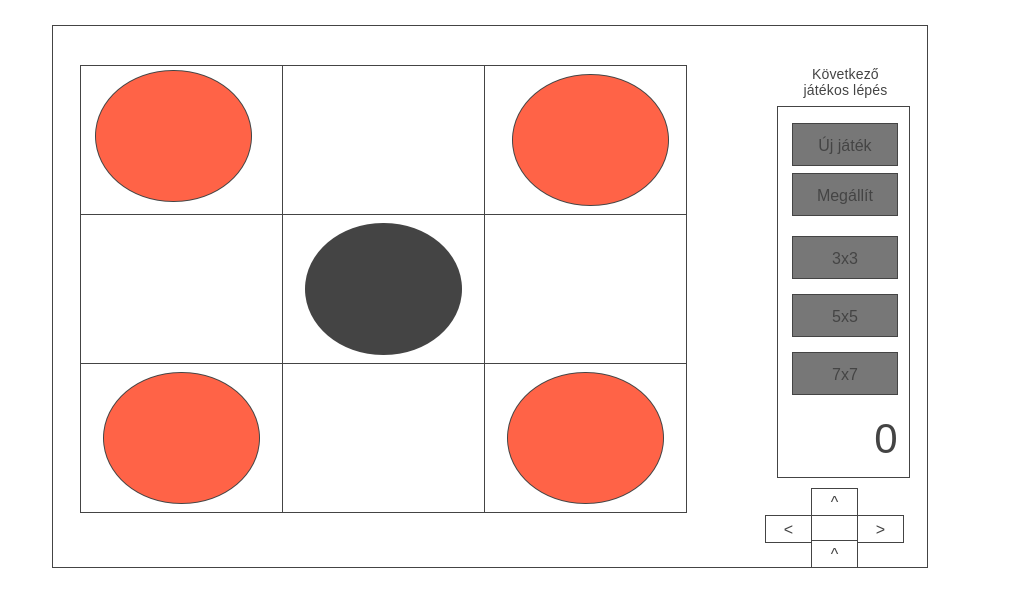
\includegraphics[width= 1\textwidth ]{MainWindow.png}
\end{center}

Ha valamelyik fél megnyerte a játékot, arról egy információs ablak tájékoztatja,
melyen szerepel a győztes fél neve és lépésszám, ami a kezdés óta eltelt.

\begin{center}
	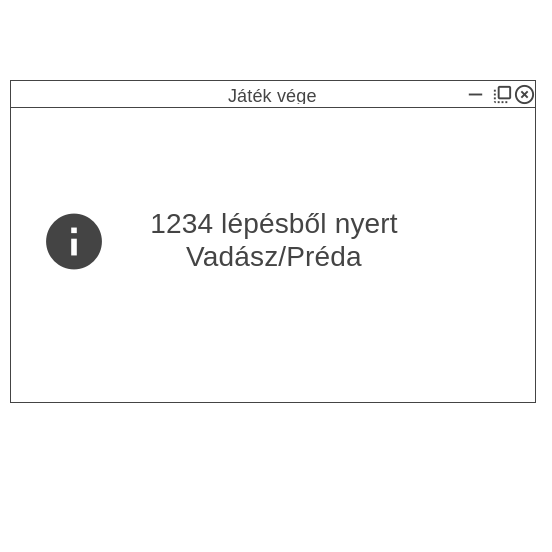
\includegraphics[width= 0.5\textwidth ]{WINdow.png}
\end{center}

A játék bármely pillanatában (kivéve ha az információs doboz aktív) van lehetőség a játék
mentésére. A Fájl -> Mentés vagy Fájl-> Betöltés gombra kattintva megjelenik a mentés ablak,
ahol a felhasználó kiválaszthatja a fájl nevét, illetve akár törölhet is korábbi fájlokat,
ha úgy gondolja, már túl sok mentés van az adott mappában.


\begin{center}
	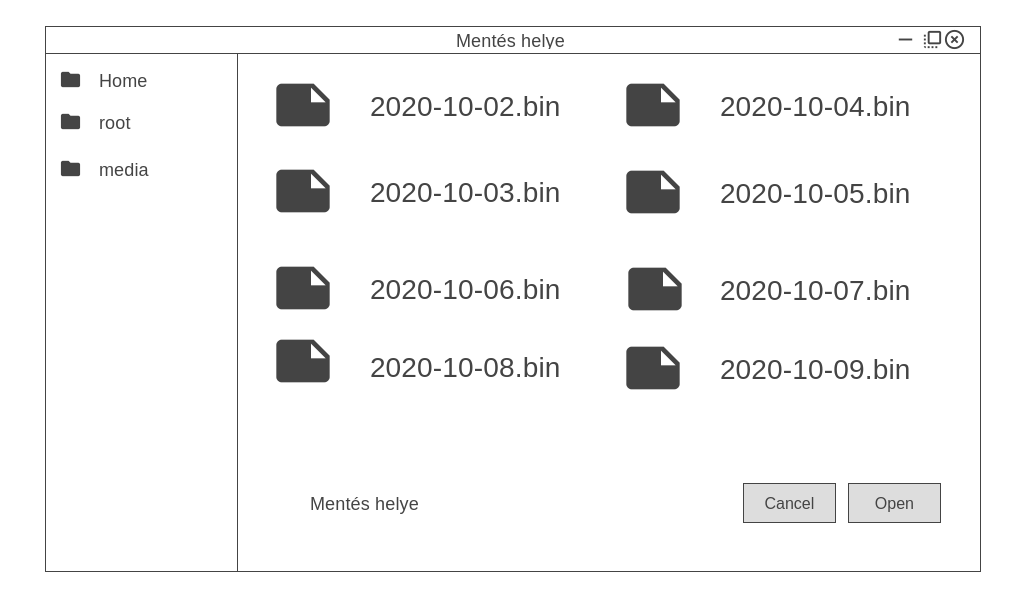
\includegraphics[width= 1\textwidth ]{Saving.png}
\end{center}

